\documentclass{article}
\usepackage[utf8]{inputenc}

\usepackage{natbib}
\usepackage{graphicx}
\usepackage[numbered,framed]{matlab-prettifier}
\usepackage{amsmath,amssymb}
 \usepackage{url}
 \renewcommand{\UrlFont}{\small\tt}
\usepackage{caption,subcaption}
%\usepackage[showframe]{geometry}
\usepackage{float}
\usepackage[ruled,vlined]{algorithm2e}
%\usepackage{algorithmic}
\usepackage{listings}
%\usepackage{inputenc}
\usepackage{listings}
\usepackage{xcolor}
\usepackage[noend]{algpseudocode}
%\newcommand{\citelink}[2]{\hyperlink{cite.\therefsection @#1}{#2}}
\newcommand\mycommfont[1]{\footnotesize\ttfamily\textcolor{blue}{#1}}
\SetCommentSty{mycommfont}
%\usepackage{tikz}



\colorlet{punct}{red!60!black}
\definecolor{background}{HTML}{EEEEEE}
\definecolor{delim}{RGB}{20,105,176}
\colorlet{numb}{magenta!60!black}

\lstdefinelanguage{json}{
    basicstyle=\normalfont\ttfamily,
    numbers=left,
    numberstyle=\scriptsize,
    stepnumber=1,
    numbersep=8pt,
    showstringspaces=false,
    breaklines=true,
    frame=lines,
    backgroundcolor=\color{background},
    literate=
     *{0}{{{\color{numb}0}}}{1}
      {1}{{{\color{numb}1}}}{1}
      {2}{{{\color{numb}2}}}{1}
      {3}{{{\color{numb}3}}}{1}
      {4}{{{\color{numb}4}}}{1}
      {5}{{{\color{numb}5}}}{1}
      {6}{{{\color{numb}6}}}{1}
      {7}{{{\color{numb}7}}}{1}
      {8}{{{\color{numb}8}}}{1}
      {9}{{{\color{numb}9}}}{1}
      {:}{{{\color{punct}{:}}}}{1}
      {,}{{{\color{punct}{,}}}}{1}
      {\{}{{{\color{delim}{\{}}}}{1}
      {\}}{{{\color{delim}{\}}}}}{1}
      {[}{{{\color{delim}{[}}}}{1}
      {]}{{{\color{delim}{]}}}}{1},
}


%\usepackage{minted} % for Julia code need to install pygmentize but I will do this later

\makeindex

\begin{document}

\begin{titlepage}
   \begin{center}
       \vspace*{1cm}

      % \textbf{Report Title: Optimizing mobility on demand with dynamic pickup station and drop of with time window}
%\vspace{0.5cm}
	 \textbf{An optimization algorithm for Dial a Ride problems in the context of intermodal route planning}
\vspace{0.5cm}

       %\vspace{0.5cm}
        %This is a tentative title
                    
       \vspace{2.5cm}

       Written by:	\textbf{Ayman MAHMOUD} \\
       Supervisors: \\
       Prof. Jakob Puchinger\\
       Prof. Asmaa Ghaffari\\

       \vfill
            
       \vspace{0.8cm}
     
       
\includegraphics[width=0.7\textwidth]{pictures/logo_nouveau.jpg}
            
       Master Ingénierie des systèmes complexes\\
       Laboratoire Génie Industrielle\\
       CentraleSupélec - Université Paris Saclay\\
       Gif Sur-Yvette - Paris - France\\
       Date: \today
            
   \end{center}
\end{titlepage}

\tableofcontents

\newpage
%\section{Acknowledgments}

\section{Introduction}


Increasing mobility demands raise the pressure on existing transport networks. Private cars, the most used mode of transport, have a particularly strong environmental impact and produce congestion. \\

Shared mobility concept existed before even the coloured television was invented. The first ride-sharing as in car-sharing program was established in $1948$ in Zurich when a housing cooperative began a small car share arrangement, it was called \lq\lq{Sefage program}\rq\rq. In this period this solution wasn\rq{t} very attractive. Simply because the automotive production got faster and cheaper and it was more appealing to own your vehicle than to share one. Many ride-sharing initiatives re-appeared in Europe afterwards but none did last until we reached the $1990\rq{s}$ when the congested traffic networks started surfacing, fuel prices risen and environmental concerns were put on the table of discussion \citep{BECKER2017}. The first bike-sharing program began in 1965 in Amsterdam, Netherlands. \\

In the current times, the rise of smartphone applications and location data increased the feasibility of shared transportation services and mobility on demand. In the region of Ile de France there\rq{s} $836km$ of accessible roads where $25\%$ experience congestion in the peak hour \cite{Traffic_france}. It is no secret that we need an effective solution. Ride sharing as in mobility on demand, can help to address these issues by increasing the number of persons per car. However, what we\rq{re} experiencing now is that, although the ride-sharing solutions exist we still have a rise in the traffic congestion and traffic density is worsening \cite{Forbes_congestion}, additionally there exists no effective method of integrating ride-sharing solutions into transport trip planners as of now, mainly due to the fuzzy and flexible nature (e.g., no fixed stops, possibility of making detours) of carpooling. Some solutions are proposed \cite{STIGLIC201812}\cite{Alonso-Mora462}, some companies actually operate on this basis but none of them is contributing significantly to the traffic congestion problem \cite{schaller_consulting}\cite{schaller_consult}\cite{Forbes_congestion}.\\  

The numbers of fleet sizing optimization are very promising, without shared mobility almost half of the taxies in Manhattan are empty at normal times, the article in Nature magazine, written by researchers in Senseable city lab\cite{senseable_city_lab}, shows that we only need $60\%$ of today\rq{s} taxis. Additionally with autonomous shared mobility, the perfect scenario, we can move all Manhattan with $137,000$ vehicles which is half of what\rq{s} on the road today \cite{senseable_city_lab}. 

To reduce the negative externalities of car travel, local governments encourage the use of public transit. Unfortunately, many suburban and rural areas are not adequately served as they lack the population density to justify public transit, i.e., the public transit is not economically viable. In cities with sprawling suburban areas, the utilization of public transit to commute to work is often low, e.g., less than $5\%$ in metropolitan areas like Houston and Atlanta in the United States \cite{STIGLIC201812}.


This report is organized as follows, in section (\ref{sec:Motivation}) I start by explaining the motivation in research into this subject, in section (\ref{sec:Methodology}) is a documentation of the methods followed in the literature review and building a bibliography, following by section (\ref{sec:literature}) where the literature in shared and intermodal mobility is discovered with the development of a conclusion and a demonstration of the gap in research that exists. Section (\ref{sec:taxonomy}) is a detailed comprehensive taxonomy that was built around the terminologies found in research papers. In section (\ref{sec:Problem_Definition}) a formal problem description and definition with a visualization in section (\ref{subsec:problem_vis}), a time sequence of events is displayed in section (\ref{subsec:timeseq}) and the problem formulation is presented in section (\ref{subsection:problem_setting}). Next, the method proposed with which the problem can be solves is presented in section (\ref{sec:Methodd}) where in section (\ref{sec:data_struc}) the data structure of the booking is presented, in section (\ref{subsec:definepickup}) we explain in details how we\rq{re} going to define the pickup stations and in section (\ref{subsec:alg}) the algorithm is shown.  We close this section with a description of the next steps for the research project in  (\ref{subsec:next_steps}) and finally in section (\ref{sec:conclusion}) is the conclusion.


\section{Motivation}
\label{sec:Motivation}

%I consider this option as a chance for me specializing in a field based on a multidisciplinary scientific approach essential to my future projects and my desire to create real expertise at the level of region of the world I come from a region strongly impacted by the transport problems, which is only a fuel that drives me to find innovative solutions in mobility.

%I want to contribute to the optimization of mobility systems around the world, to contribute to the future of mobility and ultimately to reduce overall journey times for passengers.

When it comes to shared mobility, my readings had raised questions that need answers, the gap between mobility on demand and public transit systems. To look into this gap I decided to read about existing problems from both sides (Public Transport and Mobility on Demand)

In the last few years, there has been a resurgence of interest in demand-responsive shared-ride systems for the general public \cite{HO_darp2018}. This has been fuelled in part by concerns for the environment; each commuter using a separate car leaves a large carbon footprint and also causes congestion in central business districts. Thus, the notion of a sharing economy that advocates a shift from car ownership to \lq\lq{mobility as a service}\rq\rq gained popularity. right now it is a billion dollar business. 

My motivation is fuelled by the fact that current mobility problems require intelligent solutions, dynamic ride sharing solutions offer great help to the daily commutes especially in the big cities, public transport on the other hand helps millions everyday to get to their destination,
there seem to be a relationship between both if we look into the first and last mile problem and areas underserved with public transport. We can safely say that both these modes are complementary, on one hand, public transport is quite sparse in some regions, ride-sharing or mobility on demand offers to reach areas with limited public transport connectivity, on another hand, the number of dynamic ride sharing relevant for a query increases when allowing routes which bring a passenger to a station where he can use public transport to continue 
his journey, this is because the passenger will be able to cover a longer distance paying less money, also gaining time because there is a reliable mobility service that will get him to the station of the public transport. \cite{FAHNENSCHREIBER2016176}

This way dynamic ride-sharing as well as public transportation benefit from this combination: by offering dynamic ride-sharing to the passengers using public transport, of course multi-modal transportation has existed as long as passenger transport itself, in the suburban areas we see Park \& go options were you can drive your private car to the main transportation node park the car and use the public transport service. But of course as shared mobility tries to solve many problems, I see a real motivation in integrating both modes and finding a solutions. Many researchers had already investigated this topic \cite{Bast_2016}, it is going to expanded in the third part of the literature review section (\ref{subsec:literature_part3}).


To begin literature had to be studied, to find the most recent findings in this topic, first starting with challenges present in shared mobility. Many competent engineers and researchers are trying to solve and come up with solutions as this is going to be expanded in Section (\ref{sec:literature}).


Mobility research is broad and can include many topics, when we talk about mobility optimization it  involves the integration of information, transportation, inventory, warehousing, material handling, and packaging, and certainly security.

\section{Research Methodology}
\label{sec:Methodology}

The literature review (State of the Art) phase can be divided into two categories, the first one is a general discovery to search for the current research trends in the intelligent transport community and research boards. The second category is more precise and technical 
to look into the mathematical and scientific problem definitions and identify the problems where there is need and requires research force.

The key contributions are the following:
\begin{enumerate}{
\item Comprehensive surveys that were published on topics of interest.
\item An overview of application areas of DARPs.
\item A detailed taxonomy of the problem variants.
\item Identification of potential research gaps.}
\end{enumerate}

Thanks to the free access that is granted by the school network I was able to reach the targeted articles without difficulties. My method of looking for information consisted on three main sources:
\begin{list}{}
\item • Scientific journals \& online tools
\item • Books
\item • Courses
\end{list}

\subsection{Scientific Journals}
My main sources of research were the journals, more specifically Transportation Research Journal, this journal that is published regularly is divided into $6$ parts, ranging from policy and practice, emerging technologies to transport and environment, 
the parts that significantly contributed to my state of the art are Parts $B$ \& $C$, this scope then got widened thanks to the online tools that I used (see in section \ref{subsec:onlinetools}). 

Part $B$ publishes papers on all methodological aspects of the subject, particularly those that require mathematical analysis while part C addresses development, applications, and implications, in the field of transportation, of emerging technologies
 from such fields as operations research. In Transportation Research Part $B$ I found the article that was recommended by my supervisor \lq\lq{A survey of models and algorithms for optimizing shared mobility}\rq\rq by Mourad et al. 2019 \citep{MOURAD2019}.

It was hard to choose between articles in the beginning, this is why my main reference to the articles in shared mobility was the survey \citep{MOURAD2019}. Then I started using some keywords into my search such as: \lq\lq{DARP}\rq\rq, \lq\lq{Multimodal}\rq\rq, \& \lq\lq{Last mile problem}\rq\rq.

\subsubsection{Books}

Books are the main reference if you want to understand correctly a scientific topic, in my early research I found many helpful references such as \lq\lq{The Handbook of Transportation Science}\rq\rq by Randolph W. Hall \cite{Randolphts} which was very helpful in the beginning to learn some basics on the traffic flow and capacity, the book helped me in working on my first traffic related project (explained in section \ref{subsec:online}), some other books that contributed to my state of the art is the Experimental Algorithms 2008 \cite{bookexpalg}, especially in the chapter of multi-criteria shortest paths search algorithms and Pareto optimality. Many other books contributed to my state of the art, the whole collection of books can be found in  \cite{my_bibliography}.


\subsubsection{Online Tools}
\label{subsec:onlinetools}

The literature review process wouldn\rq{t} have been possible without the very powerful online tools such as ScienceDirect that helped me widen my research by suggesting $6$ related articles to the paper I am currently investigating.
Google Scholar web search engine tools helped me to find many articles, know where it has been cited and published. This tool also showed me the researcher profiles and who they have collaborated with, their most cited work and their research topics of interest. Finally ResearchGate that helped me by suggesting papers of interest and follow the updates of the researchers in the field.
Semantic Scholars also helped my literature review because it shows a number of scientific papers and articles that were highly influenced by the actual paper I am reading.

Tools are also used to help and organize my references, in addition to the cloud drives I use to keep my research available remotely, I use Zotero, which is a tool that helps collect, organize and cite my research. Zotero also has an extension to the browser that helps collecting citation and articles directly from the web browser. 

\subsubsection{Conferences}

The mobility program was a bootloader for my research project, this conference, that had place in Pascal institute, gathered for three weeks internationally recognized experts to talk about their work on mobility, in their respective fields. I attended all the talks my schedule allowed me to attend and discussed topics on current mobility problems with many researchers and documented the presentations from my point of view.(see in references \cite{mobility_program} for additional information) 

  
\subsection{Courses}
\label{subsec:online}
Thanks to the open source material online, we can easily find the tools that can help advance in the topic.

I was advised by the program director to start a class online on the queuing theory, \lq\lq{Queuing Theory: from Markov Chains to Multi-Server Systems }\rq\rq Queuing theory aims at modelling waiting or blocking phenomena. To be more precise, in queuing theory, those phenomena are characterized by mathematical models. This makes it possible to compute average system performance such as an average delay or a blocking probability. Reciprocally it is possible to dimension system resources in order to reach a given performance level.

This online class gave me a better understanding of the queuing modelling and applications in mobility problems, this basic understanding helped me working on my first project to simulate the traffic on a road with three lane and tolling stations and then study the 
possibility of creating a traffic jam based on the rate of generation of vehicles.


In addition to this, the masters program fits perfectly the technical knowledge I need to advance in my research, just in this first semester I was able to recognize and deal with many optimization and operational research problems. 
What\rq{s} even more interesting is that most of the work we do in the class most of the times is on a subject related to mobility as an example in the modelling class the project was on traffic modelling using a hydromatic analogy and the law of conservation of flow.


Attending the class of \lq\lq{Optimization for Transportation}\rq\rq the lectures were very helpful to have a wider understanding of the modelling of the transportation problems, the dynamism of the problems and the algorithms used to find an exact or heuristic solution. 
The project of this course was one of the most interesting projects I worked on. This project gave me an insight on how to practically solve these transportation problems using powerful optimization tools such as CPLEX, the goal was to find the optimal solution of a capacitated vehicle routing problem (G-VRP) to minimize the total distance covered by the fleet. In this project I implemented my first Clarke \& Wright Savings Algorithm to find a meta heuristic solution to the routing problem.


\section{State of the Art}
\label{sec:literature}


Some leading laboratories already have a remarkable research output. In the beginning I didn\rq{t} go very far in my research and started with literature from the Industrial Engineering Lab in our school, some strong research was conducted on many mobility problems, benchmark studies and surveys. 

What came most useful in the start is the survey on model and algorithms in shared mobility \cite{MOURAD2019}. That was a comprehensive survey to the most recent variants of the shared mobility
problems, and a study of their different features and modelling approaches, not only that but the survey also explained all the constraints researchers consider into their shared mobility problems such as Time Constraints and Capacity Constraints, the relationship between transporting goods and people, pick up and delivery problems and the potential merge between both worlds. 

Strong research also came from the lab in the social and economic impacts of autonomous shuttles for collective transport \cite{antonialli2019}, some strong research also came from the lab in vehicle routing problems and new mobility services \cite{VOSOOGHI201915}\cite{vosooghi2019}.

In this topic some notable researchers had a significant contribution, one of them is: Gilbert Laporte who is currently a Full Professor of Operations Research at HEC Montréal. He has a notable contribution to the vehicle routing problem (VRP) \& Dial-a-Ride Problem (DARP). His work has been cited over $60,000$ times \cite{gilbert_laporte_profile}.

In many countries around the world there are strong research entities, operational research and mobility companies and individuals that are solving transportation optimization problems. Starting from the west, in the United States, the origin land of Uber \& Lyft, the number of research output in the mobility and transportation research is very high, in Europe we have many labs and institutes focusing on this subject with the goal of optimizing freight a people transport in the old continent especially because we\rq{re} going to witness an increase of $+42\%$ in passenger mobility and $+60\%$ in freight transport by $2050$ \cite{report_EU_2050}. In Asia the research output is very high as well.



% Solutions in shared mobility: 

\subsection{Shared mobility}
\label{subsec:Shared_Mobility}

Shared mobility concept as mentioned before contains many variants and characteristics, a great visual representation of the characteristics of the problem is presented in \cite{MOURAD2019}. In this report, we\rq{re} interested in Dial-a-Ride problems that are concerned with the following variants; mobility on demand (MoD), pre-arranged and real-time bookings. To be more specific we\rq{re} interested in DARP problems concerned with the first and last mile problems in multimodal commutes. A survey of dial-a-ride problems by Ho et al. \cite{HO_darp2018} presented an up-to-date review of recent studies on dial-a-ride problems (DARPs) with their different variants and solution methodologies. 

What is the Dial-a-Ride Problem? The dial-a-ride problem (DARP) generalizes a number of well studied vehicle routing problems such as the Vehicle Routing Problem with Time Windows(
VRPTW) and the Pickup and Delivery Problem (PDP). The DARP is a demand responsive transportation service, which arises for example in the context of patient transportation.
It is a service for elderly or handicapped people, where patients have to be delivered to medical facilities or carried back home leading to specified pickup and delivery locations. The transportation requests have to be completed under
user inconvenience considerations by a given fleet of vehicles. Assigning vehicles of a fleet to given transportation requests is usually modelled in terms of a static DARP, which has obtained noticeable attention in the literature \cite{Ritzinger_Puchinger2016}.

Another variant of the ride-sharing problem is the shared-taxi problem as a multi-vehicle dynamic DARP. In the shared-taxi problem, passengers indicate their desired pickup and
drop-off locations, their earliest/latest acceptable pickup/drop-off time, and a maximum trip time. Which means this problem shares the same characteristics, such as demand-responsiveness, as the DARP. 
However, the main difference is that most shared-taxi services aim to minimize the response time to passenger requests whereas dial-a-ride systems aim to minimize vehicle operating cost by reducing
the number of vehicles used to serve given passenger demands.

Many approaches are adopted to solve the dial a ride problem, each with a specific design that makes each problem different than the other. The most popular objectives of DARPs are to minimize service provider’s operating costs (e.g., total transportation time, total distance travelled by the vehicles, total route duration, the number of vehicles required, and driver working time) and/or users’ inconvenience metrics (e.g., total ride time, user waiting time, and deviations from requested pick-up/drop-off time windows).; this can be done by cutting down the number of fleet and maximize the occupancy rate. However, some solutions take in to consideration the social welfare and the balance of affecting ride to drivers which makes the optimization relative to the context. A small proportion of work considers vehicle emissions as well. Other more problem-specific objectives include optimizing passenger occupancy rate, cost-effectiveness metric, operator’s profit, staff workload, and the reliability of the system.

One of the proposed solutions are hybrid solutions frameworks for solving the DARP in \cite{Ritzinger_Puchinger2016}, this  includes two algorithmic components: dynamic programming (DP) and Large Neighbourhood Search (LNS). Branch \& Cut algorithm is used in \cite{Cordeau2006} to find an exact solution using an LP model. Using re-optimization and an efficient network mixed-integer optimization formulation along with simple heuristics in \cite{Bertsimas2018}, they were able to find solutions for large scale problems with $5000$ taxis and $26,000$ bookings. Some researchers used an insertion algorithm for a DARP problem with narrow time windows \cite{HAME2011}. The consideration of narrow time windows means that the vehicle route is restricted by relatively strict time limits for pickup and delivery of each customer. Narrow time windows emerge in real-time dial-a-ride services, in which each customer is given an estimate or guarantee regarding the pickup and delivery times in the form of time windows. 
These time windows are examined as hard limits to be met by the vehicle, which is not the case for most of the existing mobility on demand services.

To read more into the history of DARP related problems in \cite{HO_darp2018} a comprehensive survey of the journal papers published since 2007. Additionally the survey has a detailed taxonomy of the problem variants, and discussion on subtleties of the classification that is going to be investigated in section \ref{sec:taxonomy}. 

More on the survey side Cordeau \& Laporte presented a summary of the most important models and algorithms\cite{2008_Cordeau_Laporte}, their work and LP model was an inspiration to the model presented in section \ref{subsection:problem_setting}.  

Standard column generation scheme applied with a classical linear objective function minimizing the total travel cost but with the objective to maximize the passenger occupancy rate was used in \cite{Garaix2010}. Much more work has been published with very satisfying results. 

In the assembly of the work, there was no clear correlation  between the nature of the trip or tours in the characteristics of Dial-a-ride problems, some work displayed the context of optimization to the elderly \citep{STIGLIC201812}, the pick-up and delivery of the passengers is completely abstract from the context in most of the articles I have read.

This nevertheless was a turning point in the literature review to start studying the nature of the problem when put into different contexts. \\

To conclude this point in one sentence we can say that Inter-modality and multimodality exist in literature but none of the literature mixes between dial a ride problems and multimodal transport although it exists in real life.

Each service has a specific context, there\rq{s} a clear lack of research output in DARP optimization problems when it comes to intermodal trip planning, it comes as a responsibility to the user to manage all the bookings. Of course there\rq{s} research in multimodal trip planning, there are also very famous mobile applications such as \rq\rq{CityMapper}\rq\rq that we use everyday to find the best transportation mode to go from point A to point B. These apps (the ones similar to CityMapper) are the closest to planning a multimodal trip in real life.

Although some of these apps will allow you to book your ride that will get you to the train station, neither the app nor the mobility on demand service provider will be responsible if you arrived late for the train. In the following figure a little application to the situation described where I want to go back to my residence in Gif-sur-Yvette because the confinement is over and we need to go back for an exam, so it is very important to be there on time, I know that I will use more than one transportation mode to get there, I choose CityMapper to plan the trip for me and choose the best multimodal trip. It turns out to get there fast, I can take an Uber from my current location to the nearest metro station of line $10$, the trip planner shows it will take $85 min.$ given how Uber works it will surely take longer than that.
% (in fig. \ref{fig:citymapper_exp})

Time window pick up in Uber is not a hard constraint (check section \ref{sec:taxonomy}) the service will choose for you the closest option, also Uber Pool option will add an additional times to the wait $T > 2min.$ to find a match, we should also consider the fact that despite that the driver might be late because of many reasons, the driver can also choose to cancel the trip, Uber will surely find a replacement within minutes or even seconds but that all adds up to the wait time. 
Also here shows the disadvantage of competition to the customer, simply because Citymapper only shows you Uber as an option at the same time there maybe a Kaptain that is much closer.

\begin{figure}[H]
\label{fig:citymapper_exp}
    \centering 
\begin{subfigure}{\textwidth}
  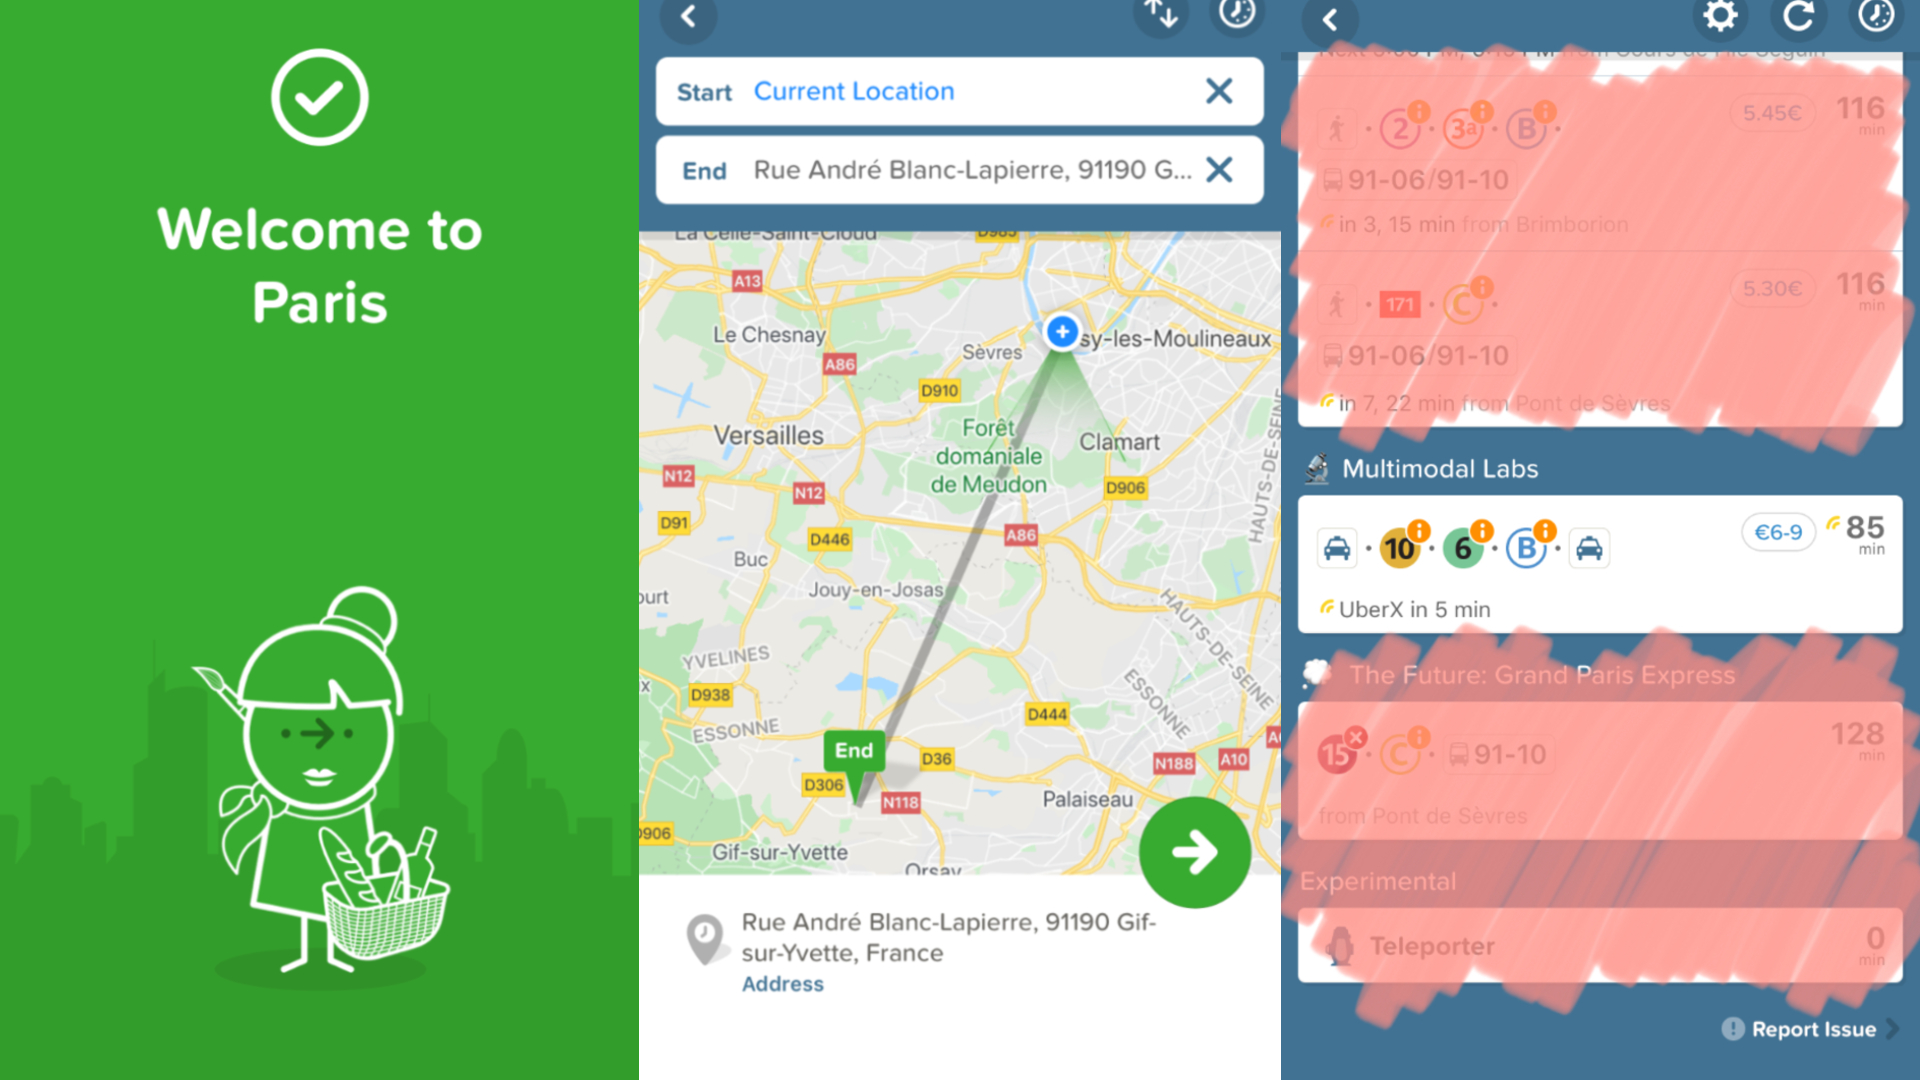
\includegraphics[width=\linewidth]{pictures/citymapper_experiment/Citymapper_experiment_1}
  \caption{From left to right: It take 5 steps to get to booking a ride on Uber}
\end{subfigure}
\medskip
\begin{subfigure}{\textwidth}
  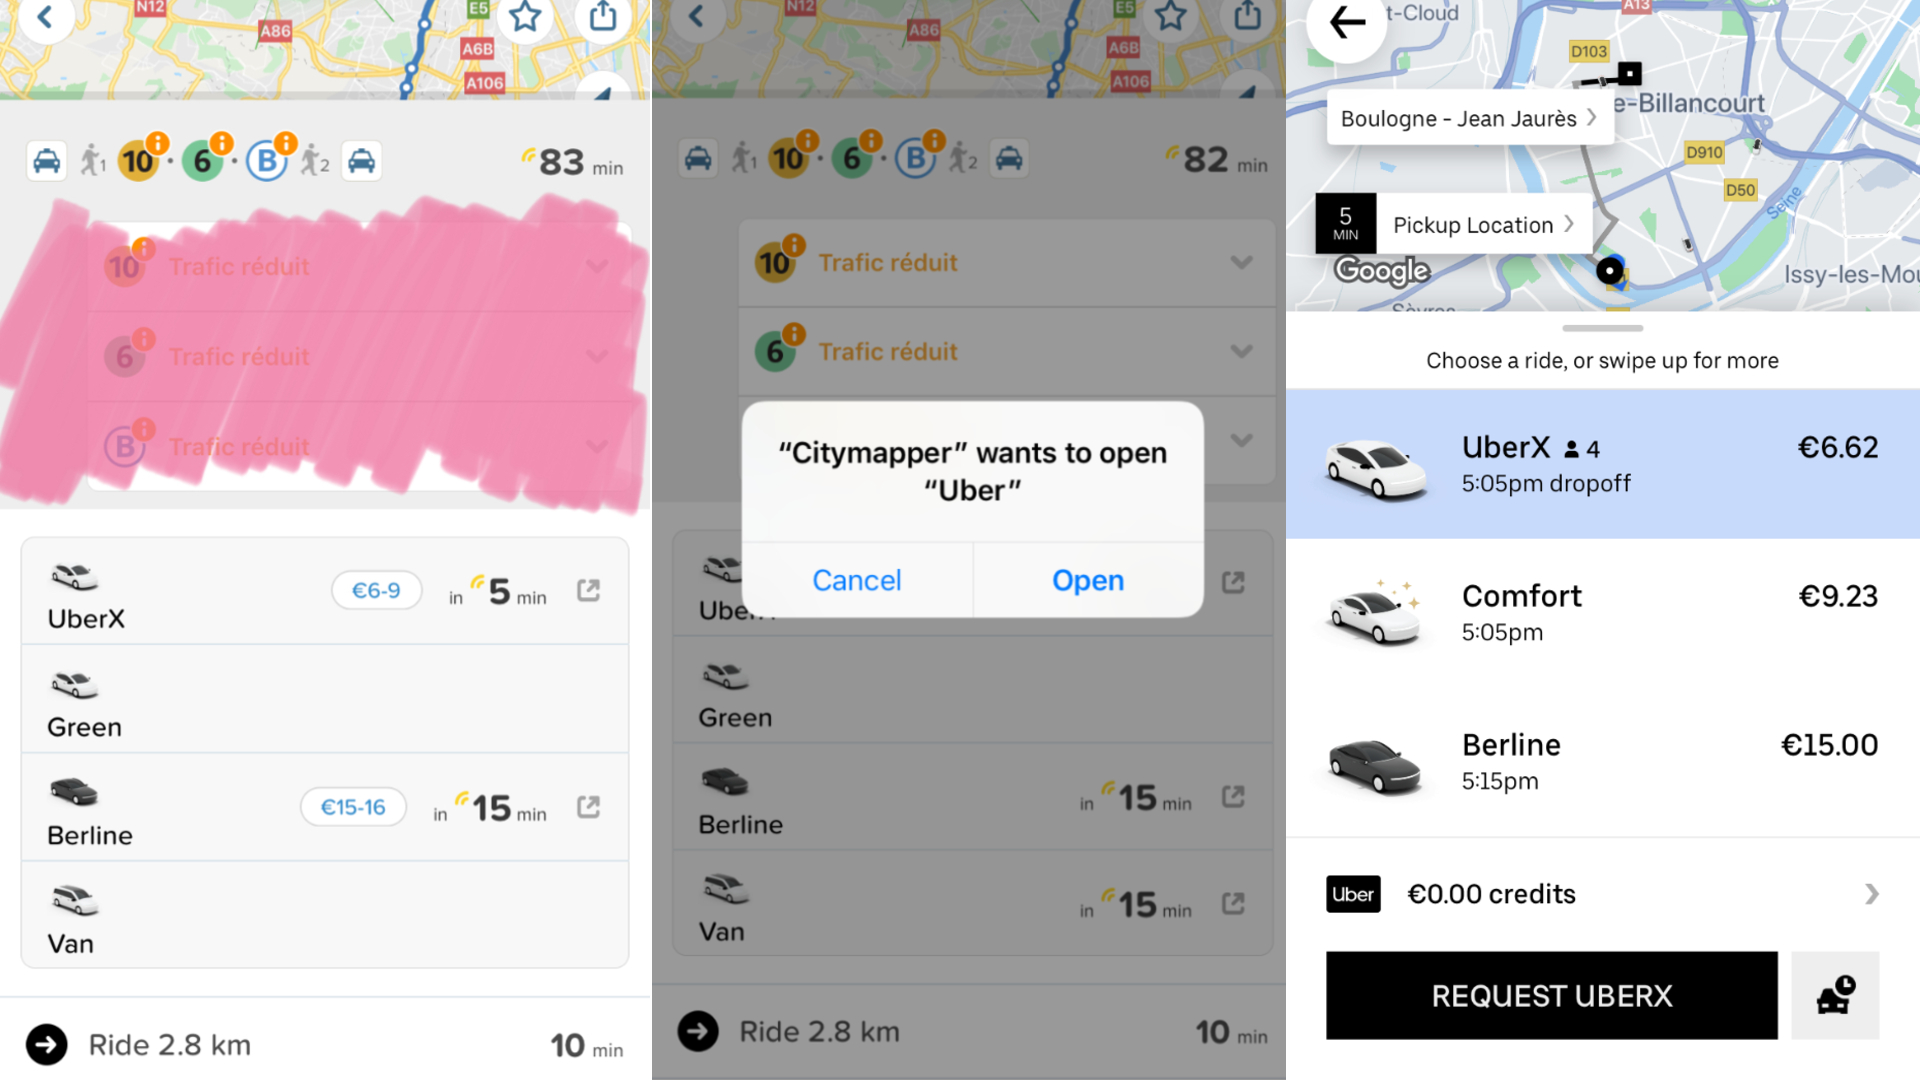
\includegraphics[width=\linewidth]{pictures/citymapper_experiment/Citymapper_experiment_2}
  \caption{As the figure shows only Uber is an option}
\end{subfigure}
\end{figure}

That\rq{s} why the state of the art took a natural turn into multimodal trip planning and routing problems.


\subsection{Multimodal Trip Planning}
\label{subsec:Intermodal}

Inter-modality, also called mixed-mode commuting, involves using two or more modes of transportation in a journey. However, the research that is going to be displayed in the next paragraph doesn\rq{t} tackle the the optimization of mobility on demand with public transport, it does mention studies that mix ride-sharing with public transport nevertheless from routing problems point of view and feasibility studies.  
One of the early notable investigation done in this area is the report \lq\lq{Ride-sharing as a Complement to Transit}\rq\rq \cite{Murray14655}, this report was published in TRB, highlights ride-sharing as an important opportunity for transportation
agencies to address the \lq\lq{last mile problem}\rq\rq, the last mile problem can be generalized to include first and last mile problems. It shows a comprehensive survey on transit agencies in the United States that are trying to close gaps in service and penetrating difficult to serve areas using ride-sharing to complement their services. The report also shows that despite these important reasons for integrating ride-sharing into transit services, only a modest number of public transit agencies is involved in ride-sharing. 

Notable research in this part is found in \citep{STIGLIC201812} where they investigated the possibility of realizing a seamless integration of ride-sharing and public transit as it may offer fast, reliable, and affordable transfer to and from transit stations in suburban areas thereby enhancing mobility of residents, they investigated the potential benefits of such a system by means of an extensive computational study.

In the paper they mentioned the ride matching technologies that are required to make it a reality, they consider a centralized system that automatically establishes matches between drivers and riders, and finally turn it into a matching rides problem where they evaluated the benefits of this integration by comparing instances of ride-matching with and without the ride-sharing service. 

Notable contribution in \cite{FAHNENSCHREIBER2016176} where they worked on combining dynamic ride sharing and public transport. In their work they address two problems in multimodality; the first is to connect public transport stations by dynamic ride-sharing and the second is connecting start and destination of a query to public station routes by dynamic ride-sharing routes, although their contribution to the subject is more on the route planning the paper proposes very good methods for ride-matching and finding connections, they also showed better connections using ride-sharing and two modes of transport in terms of travel duration and cost.% Their matches are added to their global travel information system. 

The paper \citep{Huang_2019} proposes a new method to merge public transport and carpooling networks for multimodal route planning, considering the fuzziness and flexibility brought by carpooling. They started by creating a model for both mode of transportation, to study the feasibility they studied all the 5-minute drive time areas computed around all train stops in Switzerland and determined the drive-time areas. Other researchers contributed by studying the same public transport feeding challenge but with autonomous mobility on demand in highly dense cities not rural areas,they presented a network flow optimization model that captures the joint operations of  autonomous mobility on demand systems
and public transit \cite{Salazar_schiffer}, their results show that an autonomous mobility on demand systems can significantly reduce travel times, pollutant emissions, total number of cars, and overall costs compared to an  autonomous mobility on demand system operating in isolation, which is a very interesting reflection because we often think that shared mobility helps improve public transport but the reciprocity is also valid.
To conclude this part all the studies show that the integration of a ride-sharing system and a public transit system can significantly enhance mobility and increase the use of public transport which is an expected result.


\subsection{Conclusion of the state of the art}
\label{subsec:literature_part3}
% une synthèse (pas de résumé d'articles séparés).
 
As previously mentioned, no study captures the interplay between multiple externalities arising from the synchronization of different modes of transportation.
To date, there exist no optimization frameworks that capture optimal coordination policies for MoD systems whilst assessing their achievable performance \cite{Salazar_schiffer}.

We can safely establish that the maturity of this subject is stagnant, this means that the topic is on the table now for a significant amount of time but the improvements and contributions don\rq{t} seem to serve the area of first and last mile problems when using public transportation.

One of the common integration options between a fixed-schedule system and an on-demand feeder systems the so-called Demand Responsive Connector (DRC) \citep{STIGLIC201812}. We can find an example of DRCs in
several US cities and observes that it is one of the most popular types of flexible transit services. Such systems typically operate within a service area and move passengers to and from a transfer point that connects to a major fixed-route transit network.

Although a research gap has been identified, and despite the fact that in \cite{HO_darp2018} they recommended a unified method for solving different DARP variants. 
Each DAR system has problem-specific constraints due to its underlying motivating application. DARP algorithms may need to be adaptable to different problem variants. For example, in this report the DARP is adapted to match rides with public transport and 
respect timetables for drop-off time windows.
% I conclude that there\rq{}s a need to research into this subject [3-4lines]
\label{subsec:reformulate_problem}
Expanding the last sentence, I am able to give a clear description of how we can reformulate the DARP to meet with Intermodality Problems, the problem as defined in literature can be divided into three parts:
\begin{list}{}
\item • Use mobility on demand as a feeder system to public transport.
\item • Ride matching problem, to create a seamless connection between timetables in public transport \& booking in MOD.
\item • Use data from previous bookings to build an better optimized pick-up and drop-off nodes.
\end{list}

In Section \ref{sec:Methodd} I am proposing an approach to solve this problem, and in section \ref{subsec:next_steps} I am explaining the next steps to be considered to create a framework to optimize this link. The idea consists of designing a set of minimum cost vehicle routes satisfying capacity, duration, time window, pairing, precedence and ride time constraints in the context of feeding a public transport system.


The literature review goes beyond this report. In \cite{my_bibliography} I built an online bibliography that is up-to-date with the latest research in this subject and other topics such as traffic congestion forecasting and the use of data in optimizing transportation, in addition to that you can also find an excel sheet that sorts down all the articles reviewed and their importance, authors, publishing journal, year and more detailed description such as the use of time constraints in VRPs.


\section{Taxonomy}
\label{sec:taxonomy}

\begin{flushright}
A train station is a station where a train stops.\\
- Then, tell me, what is a workstation?
\end{flushright}


A very interesting presentation of the terminology used in shared mobility can be found in\cite{hyland_taxonomy} \cite{MOURAD2019}  \cite{Schnee2009}.

\subsection{Terminology}

Besides indicating where a transportation request needs to be picked up and where it should be transported to, a shared trip must also indicate when this process can take place. 
This is usually done by associating a time window with each transportation request, whether for a passenger or freight. 

In intermodal itineraries, the goal of the passenger is to use on demand mobility service (e.g. van-pooling service) to get to the main transportation method (e.g. a train) 


A very interesting \textbf{time constraint} description, In ride-sharing systems, the time window is usually given by each passenger indicating the earliest departure time from his origin and the latest arrival time at his destination.
There could be added restrictions on the duration of the shared trips. Time constraints can also be called scheduling constraints. They are considered most of the time soft constraints, because violating them might not detach vehicle routes or intercept the flow, but it may result in passengers arriving late to their destinations, especially in real-world conditions. Violating these
constraints as mentioned in the reference may thus be allowed if it increases the likelihood of finding a solution, but discouraged through
a penalty cost \cite{MOURAD2019}. However, in the problem formulation in section \ref{sec:Problem_Definition} we present time constraint as a hard constraint.

\textbf{capacity constraint} is a factor that prevents a shared transportation resource from being overused. In ride-sharing systems, a capacity constraint limits the number of passengers sharing the same vehicle at the
same time to the number of vacant seats in that vehicle which is very important in our application to ensure each confirmed booking has a spot in the vehicle\cite{MOURAD2019} .

A taxonomy is introduced for classifying vehicle fleet management problems to inform future research on autonomous vehicle fleets \cite{hyland_taxonomy}. Their paper reviewed the
existing categories to classify scheduling and routing problems, then refine some of them as they relate to the autonomous vehicle fleet problem, what is most relevant to present in this report is their reformulation of the \textbf{time constraint} taxonomy.
They repurpose and rename this taxonomic category and in doing so remove the pure vehicle scheduling problem option and reduce the ambiguity of the time unspecified option. 
The updated  category, time-window constraints, some of the elements it includes are: 
\begin{list}{}{}
\item • No time-windows
\item • Explicit time-windows
\item • Implicit time-windows
\item • Explicit and implicit time-windows
\end{list}

The difference  between explicit and implicit time-windows manifests itself in the mathematical formulation of the problem. Explicit time-window constraints are hard constraints on the problem’s objective function; whereas, implicit time-window constraints are placed in the objective function.
 

In the thesis of Mathias Schnee with the title \lq\lq{Fully Realistic Multi-Criteria Timetable Information Systems}\rq\rq introduced and clarified basic terminology from which it is relevant to present \textbf{Footpaths} it is when sometimes a passenger has to walk short distances, like from the long distance platform to the one for local transport, or from the railway station to the bus station in front of it. A passenger may use any footpath at any point in time. This makes a footpath very different
from all other means of transportation, which may only be used at specific points in time, namely when the corresponding train departs from the station\cite{Schnee2009}. The footpath duration (transfer time) is taken into consideration in the problem formulation.

Quality of service is also mentioned in the references and it represents all the constraints that cannot be directly related to a performance factor like time constraints, it is a group of quality related objectives, a good example to explain how we can improve the quality of service for a ride sharing service is the distance between the booking location and the pickup station.  


\subsection{Pre-arranged, real-time bookings}

In prearranged ride-sharing, travellers’ demand (drivers and riders) is known beforehand (i.e. travellers\rq origins, destinations, and departure and arrival times are given in advance) and can thus be used to plan their shared trips. A real-time ride-sharing system aims to bring travellers together at short notice. Furthermore, a real-time ride-sharing system might need to be re-optimized at regular intervals as more travellers enter or leave the system, on the other hand if all the booking are specified and fixed in advance the problem becomes a pure vehicle scheduling problem \cite{hyland_taxonomy}.



\section{Problem Definition}
\label{sec:Problem_Definition}

\subsection{Introduction}

The Dial-a-Ride Problem (DARP) consists of designing vehicle routes and schedules for $n$ users who specify pickup and delivery requests between origins and destinations. 

The aim is to plan a set of minimum cost vehicle routes capable of accommodating as many users as possible, under a set of constraints.

Several local authorities are setting up dial-a-ride services or are overhauling existing systems in response to increasing demand such as BVG BerlKönig \cite{BerlKonig}, and Flinc ride-sharing \cite{Flinc}, to better describe the problem is illustrated in ( fig. \ref{fig:Diagram}) in section (\ref{subsec:problem_vis}).

The dial a ride problem often receives the pick up and drop-off time windows as inputs from the users, for mobility on demand the pick up location is usually the nearest point to the customer, in this problem we\rq{re} going to introduce dynamic pick up locations taking into consideration the drop-off time windows which we\rq{re} going to represent in our framework as timeslots and fair walking distance between customers.

In this DAR problem the drop-off time window is defined by the timetable of the destination and not by the user, which makes the whole experience more reliable and seamless (problem visualisation and example can be found in section \ref{subsec:problem_vis}). 

% problem visualization

\subsection{Problem Visualisation}
\label{subsec:problem_vis}

\begin{figure}[H]
\centering
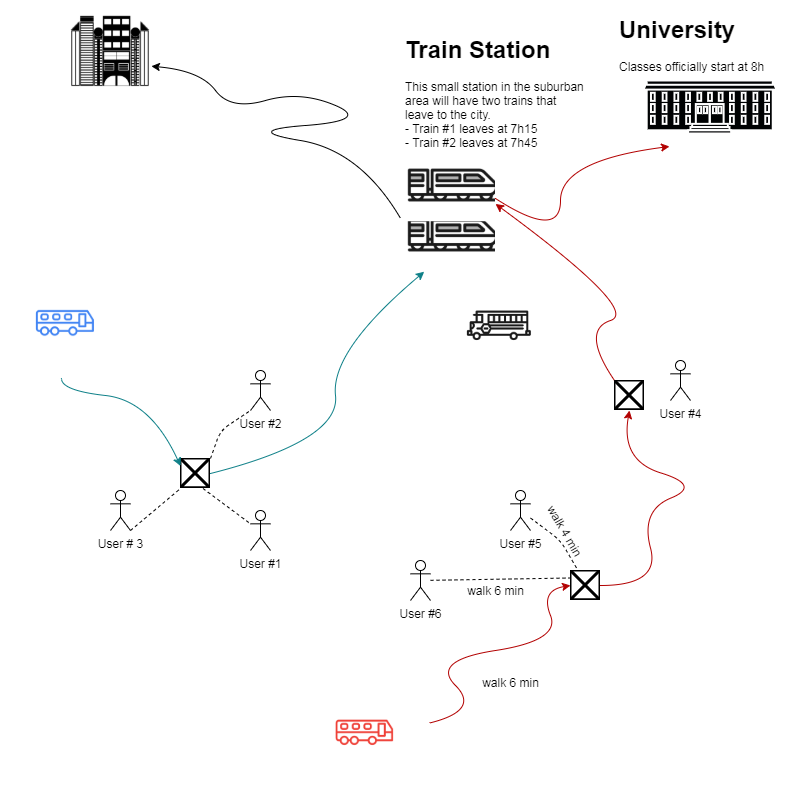
\includegraphics[scale=0.4]{pictures/Display_problem}
\caption{A comprehensive visualization of the problem}
\label{fig:Diagram}
\end{figure}

In Figure \ref{fig:Diagram} a visual representation of the problem is displayed. In this small example we have a fleet of three vehicles $\{blue,red,black\}$, a total of $6\ users$ and two possible drop-off destinations $\{Train Station, University\}$ the capacity of the vehicles are limited but the best scenario is to pick up all $6$ clients with one vehicle if this doesn\rq{t} violate any constraint. This setting represents a basic dial-a-ride problem in the morning in a small suburban city, Users $\{1,2,3\}$ work in the city and they start work at $8:00 \ am$ so they all need to catch $train \#1$ that leaves the station at $7:15 \ am$, they all live nearby so the blue vehicle will pick them up from one pick up station that is within walking distance between the three of them. Users $\{5,6\}$ go to the university that is not very far from where they live so the vehicle can drop them off right at the destination, classes start at  $8:00 \  am$ so the red vehicle will pick them up from another pick up station  that is within walking distance between the two of them, another user  $\{4\}$ requests a ride to go to the train station, $train \#2$ leaves at $7:45 \ am$, the red vehicle can pick user $\#4 $ on the way to the university a drop him off before that
$train \#2$ leaves the station, for user $\#4 $ if there are many possibilities to pick him up we choose the one that will affect the least the initial planned trip, we can measure this disturbance with a distance deviation or additional ride time added to the trip.


Of course with this small example the solution can be done on paper, but let\rq{s} imagine the same situation with $50$ bookings and a fleet of $8$ vehicles it then becomes a quite challenging task, this type of ride is called many-to-one which describes the rides from many pickup locations to one final destination. However, in this problem there\rq{s} a chance we have more than one drop off station as in the case of the red vehicle.

In the following section I am going to present the problem in a mathematical model and present all the official problem statement.



\subsection{ Problem Formulation}
\label{subsection:problem_setting}

\subsection*{Problem Statement \& Mathematical Description:}

\subsubsection{Introduction}
Although with respect to sequence the problem can be divided into two separate parts, we don't neglect the fact that all the problem can be represented and formulated in a single mathematical formulation which, in the context of optimization, can lead to a more optimal solution. This path has not been taken for the reasons listed below:
\begin{list}{}{}
\item • The mathematical model that can formulated to solve this problem will be quite large and I will risk not including all the constraints.
\item • Based on my current level of coding in Python, the work on the coding will be much clearer if the problem is formulated in two sub-mathematical formulations.
\item • Based on the rhythm of work chosen during the semester it was a wiser choice to handle each part separately in order to get separate results instead of working on a big model and keep the results to the end, it was a micro lean programming cycle. %you can input the lean programming startup figure here
\end{list}

Following these arguments the problem formulation is going to be presented in two mathematical models; the first is going to handle the first part which is the station allocation problem and the second formulation for the driver allocation problem. We can now state that in this context the problem represented is twofold.
Firstly we tackle an allocation problem where we try to minimize the pickup locations by matching the requests corresponding to the same time window with a nearby pick up station. Once the pickup stations are determined the problem transitions into a many to one dial-a-ride problem with time windows, many-to-one are generalized dial-a-ride problems with an edge. All bookings realized are destined to reach the same end destination with respect to the timeslot chosen, the solution approaches are in section (\ref{sec:Methodd}).


In section \ref{subsec:next_steps} I will discuss the possibility of formulating the problem into a single mathematical model which then can be optimized in one take and discuss the pros and cons of taking this step in my view.

This part is represented as follows, a simple formulation for the sets included in the data, then in section \ref{sebsec:st_alloc} (part $1$ of the problem), we will represent a linear programming model to minimize the number of pickup stations, following in section \ref{subsec:darp} (part $2$ of the problem) we will represent the linear programming model to minimize the number of service vehicles and total distance travelled.

%In this part we will describe the problem only at peak hours when the mobility on demand is only serving a many-to-one (Many pick up stations to one drop-off station), in the case of normal operating hours, the service runs a generalized 
%mobility on demand service where its mathematical model can be found in the following paper. \citep{2008_Cordeau_Laporte}


% time sequence
\subsubsection{Time Sequence}
\label{subsec:timeseq}
This model should also serve as a normal shared mobility service, unlike services provided by Mobility on Demand services, the requests are not served as soon as possible. However, the customer is only picked up when to ensure his arrival to destination, 
if we have a request $P_i$  it should be confirmed by the user before the pickup should have place $M_i$, which leads us to expand the time variant, since there are a lot of times involved. In figure \ref{fig:sequence} the correct sequence of events in the case of a single pick up station, and in figure \ref{fig:sequence2} an expanded sequence where we have more than one pickup station :
%$T ={ \{x\}}_{x \in \{P,M,D\}} {\{1, ..., y\}}_{y \in \{n,m,s\}}$ , with this logical development we can express the following inequalities: \\ 
%\begin{equation}
%\begin{array}{l}
%{T}_{x \in P, y \in [1,n]} + W < {T}_{x \in M, y \in[1,m]} + C < {T}_{x \in D, y \in [1,s]},\\
%W \in [0,Time_{dl_{i}}],\\
%C > 0
%\label{eq:time_constraint}
%\end{array}
%\end{equation}

\begin{figure}[H]
    \centering 
  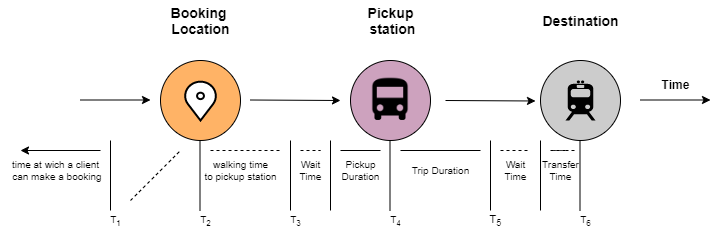
\includegraphics[width=\linewidth]{pictures/Time_sequence}
  \caption{From left to right: the sequence of events with respect to time in the case of a single pickup station}
\label{fig:sequence}
\end{figure}

\begin{list}{}
\item • \textbf{$T_{1}$ :} cut-off time after which clients cannot book anymore for a timeslot.
\item • \textbf{$T_{2}$ :} Time at which the client should start leaving his(er) location and go to the pickup station.
\item • \textbf{$T_{3}$ :} Time of arrival at the pickup station.
\item • \textbf{$T_{4}$ :} Time of beginning of the trip.
\item • \textbf{$T_{5}$ :} Time of arrival to destination.
\item • \textbf{$T_{6}$ :} Time the train trip starts.
\end{list} 

\begin{figure}[H]
    \centering 
  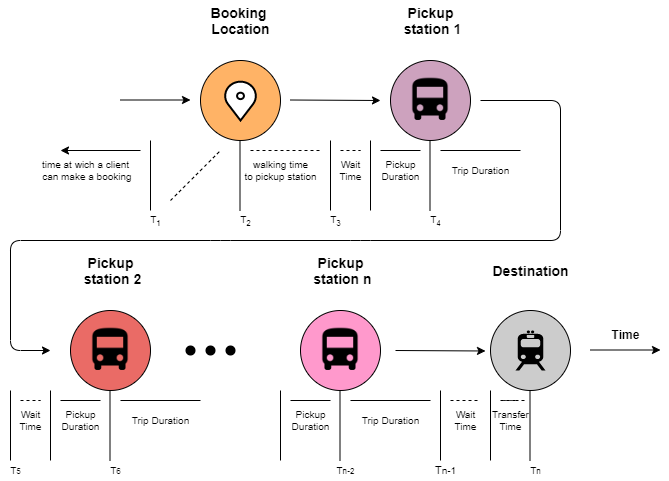
\includegraphics[width=\linewidth]{pictures/time_sequence_with_manystations}
  \caption{From left to right: the sequence of events with respect to time in the case of multiple pickup stations}
\label{fig:sequence2}
\end{figure}

In figure \ref{fig:sequence} we displayed a logical time sequence of the process starting from booking a trip until arrival to destination. Walking time to pickup station varies depending on the distance between the client (booking) location and the 
pickup station. It can be equal to zero if the station is right at where the client is located. In case of early arrival to pickup station the client can wait until the vehicle arrives to start the trip. Pickup duration is the duration the clients will take to embark 
on the vehicle and it is a constant, the trip duration varies depending on the distance between the pickup station and the destination. If the vehicle reaches destination the clients can wait at the destination until the second trip starts. Finally the transfer time 
is the time the client will take from disembarking the vehicle until reaching his second mode of transportation. As we can notice in figure (\ref{fig:sequence2}) the process (sequence) can accommodate multiple pickup stations as long as al constraints are respected.

We denote the parameter $W$ that represents the time for the client to leave his actual location and reach the pickup station, $W$ can be equal to zero if the pick up station is right where the 
customer is located. We denote also $C$ which is a contingency variable that takes into consideration many factors: \\
% it can be $ W: W = maximum(dl_{i_{1}},...,dl_{i_{n}})$ where $n$ here is the number of the people that will be picked up from the pickup station.
\begin{list}{}
\item •  Pick up duration that is proportional to the number of clients being picked up at the station.
\item •  Transfer time which is the time from the drop-off station until reaching the destination.
\end{list} 



\subsubsection*{Problem formulation}


Consider a set of $n$ number of users (or requests), $b$ number of vehicles in the fleet, $m$ is the number of pickup stations available and $s$ is the number of stations the customers can be dropped-off at (These stations must have clear and predefined timetables such as train stations and Educational Institutions). $P = \{ 1, ..., n \}$ is the set of pick up requests, $L = \{ 1, ..., n \}$ are the respective locations, $D =  \{ 1, ..., s \}$ is the set of drop-off stations,  $M =  \{ 1, ..., m \}$ is the set of pickup stations, and $B =  \{ 1, ..., b \}$ is the set of vehicles available.

For simpler model formulation we will change the size of $D$ to be equal to the size of $P$, in the context of this problem $D = \{1,2\},\ 1 = Train Station,\ 2 = School$. The new formulation of $D$ is as follows:
\begin{equation*}
\begin{array}{l}
D = \{1, ..., m\}\\
where\ D_i = \{1,2\}, \ i \in M \\
1 = Train St.,\ 2 = School \\
 \implies s = m 
\end{array}
\end{equation*}

\subsubsection{Part I: Station Matching Optimization}
\label{sebsec:st_alloc}

The first part can be represented in the form of a classical facility location optimization problem, the idea is that we have a set of potential pickup stations (  $M =  \{ 1, ..., m \}$ ) and we choose the best among these potential stations to open and receive bookings, this choice is of course subject to constraints requiring that all booking must be services by the established stations.The objective is to minimize costs, the cost here is directly proportional to the distance between the actual location of the bookings and the pickup stations. OR. these typically include a part which is proportional to the sum of the distances from the demand points to the pickup stations, in addition to costs of opening them at the chosen sites.

\label{sec:walk_limit}
As we can see this is an optimization problem where the pick up will be realised by a cluster of demands sharing the same geographical area, there will be a designed algorithm (in section \ref{subsec:alg})
that calculates the location of the best virtual pick-up station, for this algorithm we will introduce a distance limit denoted by $dl_i$ which is the maximum distance the customer is willing to make to reach the pick up station,  because when transporting passengers, reducing user inconvenience must be balanced against minimizing operating costs. The optimization problem is visualized in the figure \ref{fig:p-median}
% remember that there is a diffrerence between explaining the problem formulation and the algorithm, here we don't need to show the list of potential stations, suffice to show the matching between both

\begin{figure}[H]
    \centering 
  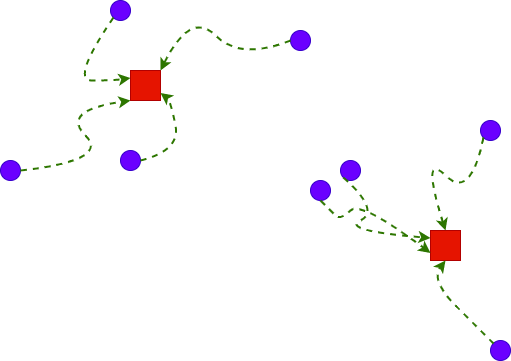
\includegraphics[width=\linewidth]{pictures/pmedian}
  \caption{blue dots are the locations of the booking and red square are the potential pickup stations}
\label{fig:p-median}
\end{figure}

The model is going to represent an uncapacitated  pickup stations where there is no limit to how many can be at the station at once.


% LP Presentation here:
\subsubsection{Model}
\label{subsection:model_partI}

Consider $n$ customers $i \in \{1,2,...,n\}$ and $m$ pickup stations $ j \in \{1,2,…,m\}$. Define binary variables $x_{ij} \in \{0, 1\}$,  $x_{ij} = 1$ if station $j$ is going to receive booking $i$, 
and binary variable $y_{j} \in \{0,1\}$, $y_{j}= 1$ if a station is open at location $j$, $y_{j}=0$ otherwise. $f_j$ is a continuous variable that describes the activation cost of stations $j$ and $c_{ij}$ is the distance cost that should not pass a certain limit.
Finally as mentioned before $dl_i$ is the maximum walking distance the driver is willing to make to get to the pickup station.
 An integer-optimization model for the problem can now be specified as follows:


\begin{equation*}
\def\arraystretch{2}
\begin{array}{lllcll} %{ll@{}ll}
\text{Minimize:}  && \displaystyle\sum\limits_{j=1}^{m}f_{j} y_{j} + \sum\limits_{i=1}^{n}\sum\limits_{j=1}^{m}c_{ij}x_{ij} && & \\
	&	&	&	&	&  \\
\text{subject to:}&   &  &  & &\\
	&	&	& 	&	& \\
	 \displaystyle\sum\limits_{j=1}^{m}x_{ij} &=& 1 &  \forall i \in \{1,2,...,n\} & & (1) \\  
	  % still \ don't know &=& 1 &  \forall  i \in \{1,2,...,n\}  & & (2) \\ 
	 c_{ij} &\leq& dl_i &  i \in \{1,2,...,n\} &j \in \{1,2,...,m\}  & (3) \\ 
	 x_{ij} &=& \{0,1\} &  \forall  i \in \{1,2,...,n\} &j \in \{1,2,...,m\} & (4) \\ 
	 y_{j} &=& \{0,1\} &  \forall i \in \{1,2,...,n\} & & (5) \\ 
\end{array}
\end{equation*}

The first constraints $(1)$ require that each customer’s demand must be satisfied.% Constraint $(2)$ provide variable upper bounds; even though they are redundant, they yield a much tighter linear programming. 
The constraint $(3)$ assures that no travelled distance by any customer passes the distance limit $dl_i$. The constraints $(4)$ and $(5)$ define that $x_{ij}$ and $y_j$ are binaries.

\subsubsection{Part II: Driver Matching Optimization}
\label{subsec:darp}

The DARP may be defined on a complete directed graph $G = (N,A)$ where:


\subsubsection*{N}

$N = P \cup D \cup \{0, n + s + 1\}$, nodes $0 \ and \  n + s + 1$ represent the origin and destination depots.
% here there was previously the walk limit paragraph

A request is a couple $(i,j)$, where $i \in N\  \& \  j \in N $ the travel time of this couple will be denoted $t_{ij}$,  consider $t_{ij}$ the trip duration from$i$ to $j$.

%The algorithm will then introduce - , $M = \{ 1, ..., m \}$ is a set of pick up stations
As mentioned $m$ the number of active pick up stations defined ($m \leqslant n$),  $(i,j)$ is a couple of a pick up station, $i \in M\ \& \ j \in M \cup D$, $M_i$ and a drop-off station $D_j$ or another pickup $M_j$.
%This couple will be represented by a vertex $v_i \in V$ to  each vertex associated the pick up time at the station. 
Let $R_i, i \in M$ the pick up time from the station and $R_j$ the pickup or drop off \textbf{predefined}, $R_i + t_{ij} \leqslant R_j$.

With each pickup node $i$ are thus associated an origin and a destination node. Each vehicle $b \in B$ has a capacity $Q_b$


With each node $i \in N$ are associated a load $q_i$ and a non-negative service duration $d_i$ such that 
\begin{equation*}
\begin{array}{l}
q_0 = q_{n+s+1} = 0, \ q_i = - q_j,\\
Where \  (i = 1, . . . , m),\ (j = 1, ... , m+s+1) \\
d_0 = d_{n+s+1} = 0
\end{array}
\end{equation*}

\subsubsection*{A}

$A$ time window $[e_i, l_i]$ is also associated with node $i \in N$ where $ e_i\ and\ l_i$ represent the earliest and latest time,
respectively, at which service may begin at node $i$. With each arc $(i, j) \in A$ are associated a travel time $t_{ij}$ .

For each arc $(i, j) \in A$ and each vehicle $b\in B$, let $x_{ij}^{b} = 1$ if vehicle $b$ travels from node $i, i \in N$ to node $j, j \in N$. For each node $ i \in N$ and each vehicle $b \in B$, let $T^{b}_{i} $ be the time at which vehicle $b$
begins service at node $i$, and $Q^{b}_{i}$ be the load of vehicle $b$ after visiting node $i$. Finally, for each group of users $i, i \in M$, let $E^{b}_{i}$ be the ride time of user $i$ on vehicle $b$.

\noindent The order of events is described in section (\ref{subsec:timeseq}).

\noindent  The mixed inter linear programming model is represented in section (\ref{subsection:model}).
% LP Presentation here:
\subsubsection{Model}
\label{subsection:model}

This problem can be represented using a three index formulation. The three index variable $x_{ij}^{b}$ is a binary variable that is equal to 1 only if the couple  $(i,j)$ is going to be served by vehicle $b$. The formulation is as follows:

\begin{equation*}
\def\arraystretch{2}
\begin{array}{lllcll} %{ll@{}ll}
\text{Minimize:}  && \displaystyle\sum\limits_{b \in B}\sum\limits_{i \in N}\sum\limits_{j \in N}x_{ij}^{b} && & (1)\\
	&	&	&	&	&  \\
\text{subject to:}&   &  &  & &\\
	&	&	& 	&	& \\
	 \displaystyle\sum\limits_{b \in B}\sum\limits_{j \in N}x_{ij}^{b} &=& 1 &  \forall i \in M & & (2) \\ %(i=1 ,..., m)% 
	 \sum\limits_{j \in N}x_{ij}^{b} - \sum\limits_{j \in N}x_{n+i, j}^{b} &=& 0	& \forall i \in M \ \& \   n+i \in N, \ b \in B	&&  (3) \\
	 \sum\limits_{j \in N}x_{0j}^{b}&=&1	&\forall b \in B & & (4) \\
	 \sum\limits_{j \in N}x_{ji}^{b} - \sum\limits_{j \in N}x_{ij}^{b} &=& 0	& \forall i \in N, \ b \in B	&&  (5) \\
	 \sum\limits_{i \in N}x_{i,m+s+1}^{b} &=& 1	&	\forall \ b \in B& & (6) \\
	 T^{b}_{j} &\geqslant& ( T^{b}_{i}+t_{ij}+W)x_{ji}^{b} 	& \forall i \in N,\  j \in N, \ b \in B		&&  (7) \\
	 Q^{b}_{j}& \geqslant& ( Q^{b}_{i}+q_j)x_{ji}^{b} 		&\forall i \in N,\  j \in N, \ b \in B		&&  (8) \\
	 E^{b}_{i}	&=&T^{b}_{n+i} -( T^{b}_{i}+W)	&\forall i \in M \ \& \   n+i \in N, \ b \in B		& & (9) \\
	 e_i \leqslant T^{b}_{i}	&\leqslant	&  l_i	&\forall i \in N, \ b \in B	&& (10) \\
	 max\{0,q_i\} \leqslant Q^{b}_{i}&	\leqslant&min\{Q_k, Q_k + q_i\} 	&\forall i \in N, \ b \in B	&& (11) \\
	 x_{ij}^{b} &\in& \{0,1\}	&\forall i \in N,\  j \in N, \ b \in B	& & (12) \\
	 E^{b}_{i} &\leqslant	&  {d}_{max}	&\forall i \in N,\ b \in B	& & (13) \\
\end{array}
\end{equation*}

As we can notice in the model the pickup has place at $i \in M$ and $m$ is the number of active pickup stations.  Let’s define the constraints necessary to solve the problem. In (1), (2) we need to make sure that each pickup is assured only once by the same vehicle,
then we need to assure that each number of bookings picked up at a station are dropped off (3).
Furthermore, in (4)(6) \& (5) each driver starts the journey (shift) from the depot station and ends the journey at the depot station as well and when a driver arrives at a given station, he needs to leave that station at some point. 
Plus, we have to take into account the times of beginning and end of shifts of the drivers as shown in(5),(6). In (7) we account for that constraint that the vehicle takes a certain time to drop off passengers or take new ones, as well as travel from one station to the next in its itinerary. We now have to make sure to respect the passengers expected pick-up and drop-off times. That why in (7) the inequality representation of the time sequence presented in figure (\ref{fig:sequence}) where the time at pickup or drop-off $T^{b}_{j}$ should be after the trip time with the contingency factors coming from $T^{b}_{i}$.

In (8) the capacity constraint where we have multiple pickup stations as shown in figure (\ref{fig:sequence2}), the number of bookings increase with respect to each pickup station visited.

Concerning the ride duration denoted $E^{b}_{i},\ \forall i \in N$, in (9) we define this duration to be equal to the sum of the time at which the booking $i$ picked up is dropped off and $W$ minus the time at which the booking $i$ is picked up. In (13) we introduce $ {d}_{max}$ which is the maximum duration a booking $i$ is willing to stay in the trip and  $E^{b}_{i}$ should be smaller than this duration.

The driver must arrive during the time frame demanded by the clients and drop them off at their destination on time. The expected time frame at station $i$ is denoted $[e_i,l_i]$, this constraint is (10).  
In (11) we take into account the maximum capacity of the buses. At all times, the driver $b$ cannot have more than $Q_b$ in his(er) vehicle.
In the next section we discuss the solutions approaches.

\section{Solution Approaches}
%\section{Method}
\label{sec:Methodd}

%\subsection{Introduction}

In this section we are going to develop our method to find a solution to this problem, as we can see from the problem formulation that the process faces two main problems. The first is a station allocation problem where we try to define and minimize the number of pickup stations and the second problem is a DAR problem where we try to minimize the number of vehicles and operational cost.


\subsection{Data Structure}
\label{sec:data_struc}

The data being used for idea validation is a modified dataset that was provided by Yuso which is a fleet management startup. The structure remained the same with some exceptions; below is a sample representation of a Booking node, each booking chooses a drop-off station and a timeslot (as an example: if a user wants to go to the train station shown in fig. \ref{fig:Diagram}, he will choose train $\#1$ and then picks timeslot $10$ that corresponds to the train leaving at $12:15am$ ). We can also notice in the following structure that the booking defines the maximum walking distance limit, in this example it is $2000\  meters$ and in the model the algorithm adapts the allocation station to ensure the booking doesn't walk more than the maximum distance to get to the station. 
\begin{lstlisting}[language=json,firstnumber=1]
"bookings": [
    {
        "id": 16566388,
        "passengers": 1,
        "maximumDuration": 2100,
        "jobs": [
            {
                "id": 23926039,
                "duration": 60,
                "latitude": 49.01606369018555,
                "longitude": 1.6916327476501465,
                "station": "s17",
                "timeslot": 10,
                "distancelimit": 2000,
                "location": [
                    32,
                    39
                ]
            }
        ]
    },
]
\end{lstlisting}

Following this the algorithm will be tested on real datasets provided from Dr. Maxime Chassaing from LIMOS Lab in France, the datasets are collected from cities all over France and the characteristics of the instances can be found in their dedicated website \cite{darp_instances}. The results are shown with the observation in section \ref{sec:results}.


% Propose algorithm here
Different solution approaches have been proposed for the DARP and its variants. Some solution approaches can apply to more than one problem type. 
For example, heuristics or meta-heuristics can be applied to solve both static-deterministic DARPs and dynamic-deterministic DARPs

\subsection{Defining Pickup Stations}
\label{subsec:definepickup}


This algorithm in section (\ref{subsec:alg}) can then be expanded to include many pickup stations on the way. The output of this maximisation will give up a binary set $x_e$ where $e \in E$, we apply the algorithm to define the set $M$ for each timeslot.

\subsubsection{Algorithm}
\label{subsec:alg}
As already mentioned, the problem complexity imposes the use of some heuristic procedure. The adopted approach is structured into two stages, the Pre-Processing Phase
and the pickup virtual station phase. In this subsection the following Algorithm \ref{alg:pickup_station} takes as an input argument the set of nodes for each timeslot. %defined by $x_e$ (feasible $(x_e = 1)$ or not feasible $(x_e = 0)$.)
In this basic algorithm we define clusters of nodes and then a pick up station is defined that should respect all the constraints. In reality there would be constraints on the pick up station discussed in section \ref{subsec:next_steps}. Currently the only constraint 
is that walking distance time of booking $i$, $i \in P$  is less than $dl_i$ which is the walking distance time limit presented in section \ref{sec:walk_limit}.

The algorithm \ref{alg:pickup_station} adopted to define clusters of pickup stations is based of a very simple approach where a set of pickup stations are already defined on the map. 

Pickup station allocation involves specifying (activating) the stations that provide demanded services there are a variety of different models to solve
this problem.
The p-median problem is a specific type of a discrete location model. We wish to place $p$ locations to minimize the average distance between a demand
node and the location in which a station is placed. The capacity constraint is neglected since it is taken into consideration earlier.

The stations that will be active are the stations that are closest to the bookings at the specific timeslot. For better illustration check figure \ref{fig:pickup_stations}.

\begin{figure}[H]
    \centering 
  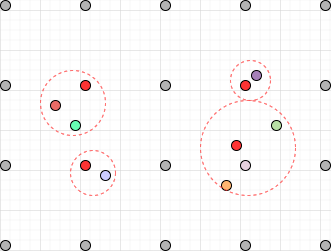
\includegraphics[width=0.5\linewidth]{pictures/pickup_stations}
%Timeslot_numbered
  \caption{grid of available pickup stations, in red are the activated ones in a timeslot}
\label{fig:pickup_stations}
\end{figure}



%Another method that can also be used is the DBSCAN method 


%the elbow method (KMeans clustering algorithm, see explanation in \citep{cluster_kmean}), when it comes to clustering, it’s hard to know how many clusters are optimal but in our case the range of $k$ (the number of clusters) is going to be supported by the value $dl_i$ and the fleet size available at timeslot $f$, we can first check the distortion which is calculated as the average of the squared distances from the cluster centres of the respective clusters, then calculate the inertia which is the sum of squared distances of samples to their closest cluster centre.

%We iterate the values of k from 1 to $k_{max}$ and calculate the values of distortions for each value of $k$ and calculate the distortion and inertia for each value of k in the given range.

%Using the elbow curve it will give us the best $k$ value, then we will go over the booking locations and calculate the walking distance limit for each location to the cluster centre to make sure no distance is greater than  $dl_i$. A simple representation of the clusters and the corresponding pickup station can be found in the problem visualization section \ref{subsec:problem_vis}


\begin{algorithm}[H]
\label{alg:pickup_station}
\SetAlgoLined
\LinesNumbered
\SetKwInOut{Input}{Input}\SetKwInOut{Output}{Output}
\SetKw{KwBy}{by}
\Input{$P$ = set of Pick up location coordinates ($ID$,$lon$,$lat$), $x_e$,$dl_i$, $F$ = set of timeslots available to drop-off, $V$ = fleet size, $M$ a set of predefined pick up stations ($ m \leqslant n$) ) }
\Output{$AM$ = index to the assigned pickup stations defined by the algorithm. }
\BlankLine
 initialization\;
AM $\leftarrow$ empty list [ ]\;
AM\_temp $\leftarrow$ empty list [ ]\;
Distances $\leftarrow$ empty list [ ]\;
  \For{$i\gets1$ \KwTo $length(F)$ \KwBy $1$}{
	pickup\_list $\leftarrow$ empty list [ ]\;
	\For{$j\gets1$ \KwTo $length(P)$ \KwBy $1$}{
		Distances $\leftarrow$  calculate\_distance\_to\_stations(P[j][$lon$,$lat$],M[:][$lon$,$lat$])\;
		}
	AM = minimize\_n\_stations(Distances, $F$)\;
	\tcp{An assignment of demand nodes to each station is made, such that the distance between a demand nodes and stations is minimum for every timeslot}
   }
\KwResult{$AM$}
\caption{Algorithm to define pickup stations.}
\end{algorithm}

%Another method of clustering bookings into central pickup stations is to set predefined pickup zones and then match bookings to the stations, the station then becomes active if and only if there are bookings matched to it (see explanation in section \ref{subsec:next_steps}).


\subsubsection{The matching problem}
\label{subsec:matching-prob}

The matching problem is a sub-problem where we have $n$ potential bookings and let $f$ denote the number of time-slots available at a drop-off station. $F = \{ 1, ..., f \}$ As an example let $F_1$ be the timetable of train $\#1$.\\
I will create a node for each booking $i \in P$ and a node for each destination timeslot $f \in F$ an edge connecting node $i$ and $f$. If there is a feasible match between booking $i$ and timeslot $f$. 
Let $T_i$ denote the time at which the booking is realized, as shown in section \ref{subsec:timeseq} it should be before the drop off time (also shown in Constraint $(10)$ in section \ref{subsection:problem_setting}).

The total trip time from pick up station until drop off is calculated:
 
\noindent$Total\ trip\ time = W + t_{ij} $, the match is possible if and only if the drop-off time of booking $i \in P$ is in a time window $[T_f - tl_i,T_f - C ]$ where
$tl_i$ is the maximum time the user is willing to wait after drop-off, for the sake of simplicity this time is going to be a constant (for example $15min$), but what can also be done is to have it defined by the client. Some clients are willing to
wait longer time than others.

Each edge $e$ has a weight that is the number of bookings per timeslot denoted by $v_e$, the matches are not unique, this means that we can have two bookings matching with two timeslots, we add the booking to the edge that has more weight as shown in figure \ref{fig:timelsot}.

%Let $E$ represent the set of all edges in the bipartite graph and let the binary decision variable $x_e$ for edge $e \in E$ indicate whether the edge is in an optimal matching $(x_e = 1)$ or not $(x_e = 0)$.

This match maximization is then going to be reflected into clusters of pickup stations, then the pick up time is defined as shown in equation (\ref{eq:pick_up_time}):
\begin{equation}
\label{eq:pick_up_time}
Pickup \ time \ at \ station\ i, \ (i \in M) = T_f - W - t_{ij} - C
\end{equation}


\begin{figure}[H]
    \centering 
  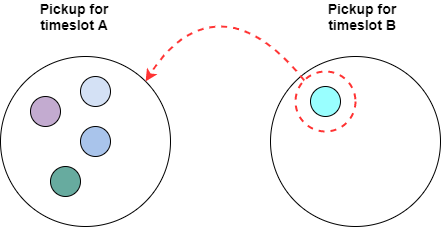
\includegraphics[width=0.7\linewidth]{pictures/Timeslot}
%Timeslot_numbered
  \caption{moving a booking between two timeslots to reduce the number of fleet if all constraints are respected}
\label{fig:timelsot}
\end{figure}


%\begin{equation*}
%\def\arraystretch{2}
%\begin{array}{llclll} %{ll@{}ll}
%\text{for each (f) :} 	&	&	&	&	&  \\
%\text{Maximize:}  & \displaystyle\sum\limits_{b \in B}v_{e}x_{e} &&& & (1)\\
%	&	&	&	&	&  \\
%\text{subject to:}&   &  &  & &\\
%	&	&	& 	&	& \\
%	& \displaystyle\sum\limits_{e \in E_i}x_e  &\leqslant& 1 &  \forall i \in P & (2) \\ %(i=1 ,..., m)%
%	&  T_f - C - tl_i &\leqslant& T_{drop-off_{(i)}}\leqslant  T_f - C	& \forall i \in P	&  (3) \\
%	&x_{e} &\in& \{0,1\}	&\forall e \in E	&  (4) \\
%\end{array}
%\end{equation*}

This approach of maximizing bookings per pickup is still questionable due to the fact that it might not be the optimal solution to move the booking from a time slot to another, it is only beneficial in the case of applying a shift that will directly reduce the number of fleet, this part is subject to testing to validate, the comparison between the results of the algorithm and the actual results of the real instances can be found in section \ref{sec:results}

\subsection{Solving the DAR problem}

The Dial a ride problem is a developed VRP with time windows, the solution approach in this part is inspired from Cordeau \& Laporte 2008 \cite{2008_Cordeau_Laporte}

\subsubsection{Algorithm}

The algorithm here is a continuation of the output of part 1 of the problem, after given the active pickup stations ...


\begin{algorithm}[H]
\label{alg:darp}
\SetAlgoLined
\LinesNumbered
\SetKwInOut{Input}{Input}\SetKwInOut{Output}{Output}
\SetKw{KwBy}{by}
\Input{$M$ a set of predefined active pick up stations}
\Output{Drivers assignments for each timeslot}
\BlankLine
 initialization\;
\tcp{The algorithm is done but not put here yet}
Objective = minimize\_total\_distance(data)\;
\KwResult{$Output$}
 \caption{Algorithm to define assignments for each driver.}
\end{algorithm}


\section{Results}
\label{sec:results}
\subsection{Introduction}
Here I am going to introduce the main features I want to show in the results.

\subsection{Optimization Environment}
The code python
the optimizer gurobi
the laptop hp .. processor...


\subsection{Comparison}

I want to create a link that shows all the results in an extensive way.
I want to show at least 4 plots and a table showing a comparison between given solutions and solutions found by mu algorithm

\subsection{Observations}
In this section I am going to discuss any data in the results that might give the wrong impression about my algorithm and explain the reason(s) behind it 


\subsubsection*{The value of time}

\begin{flushright}
We often forget that the most valuable asset for humans is time.
\end{flushright}

Coming to the end of this report, the question is why is this a valuable feeding system to public transport?
The answer is twofold. 

Because people had shown the incapacity to manage their time correctly, this is due to the fact that we\rq{re} unaware of the all the fluctuations happening that might be a changing factor in our trip time, if we want to make sure we don\rq{t} miss our train we always put a contingency additional time that will allow us to reach before the time limit within a safety margin, this safety margin differs from one person to another, some people exaggerate and arrive too early, some people get lucky and arrive on time, other people fail to 
make it in time. The system will help the three types. 


In addition to that, if we optimize this system we might prove that we don\rq{t} need all these shared mobility services, shared mobility research in big cities such as Berlin and New York showed us that we don\rq{t} need all these
taxis circulating around (see section \ref{sec:literature}), numbers showed we need $40\%$ less taxis in New York, Manhattan area. Planning these first and last mile commutes for the customers who are using public transport will help them gain time and save money.


\subsection{Next Steps}
\label{subsec:next_steps}
The first step in the problem definition statement is to be able to present the work in a mathematical formulation, the LP model and Algorithm in \ref{subsection:problem_setting}  are a preliminary representation of the work, the DARP part is very similar to the YUSO project in ST7, so I will use a similar model to optimize the LP model in \ref{subsection:problem_setting}, ride matching problem, also an LP model is going to be implemented using CPLEX, to create a seamless connection between timetables in public transport \& booking in MOD. The pickup station should not be the cluster centre, simply because we have constraints on where the station can be located, as an example the pickup station cannot be in a private property, or at a busy street.
These constraints are set by knowing the demography of the city the service is operating in. The data that is going to be used in this problem is the \textbf{modified} YUSO project data that you can see a sample of in section \ref{sec:data_struc}. \\


Next steps to explore include the following:
\begin{list}{}
\item • Create a mathematical formulation for the whole model
\item • Optimize the whole model (instead of dividing it into two part) and compare results
\item • Create user profiles for daily commuters to optimize routing.
\item • Merge real-time booking with prearranged booking.
\item • A framework of ride-sharing algorithms to build the most efficient public transport feeder.
\item • Quantify the benefits in saving time with real data. 
\item •  How such a model can impact future transportation systems.
\item •  Merge between real-time and pre-arranged bookings.
\end{list}

Better route planning comes with better data, the idea is to have the most amount of input to the problem the earliest possible, in order to be able to better allocate clients to drivers and better choose the pick up stations.The optimization problem will affect globally the operation cost. The cost saved can be reflected in the total ride cost, which will be a great incentive for the customers to book their rides earlier.


\section{Conclusion}
\label{sec:conclusion}

This report reviewed different problems of shared mobility in multimodal systems and mobility on demand systems along with their solution approaches.Then in the report I presented a case studies 
analysing shared mobility system performances or studying their potential impacts on people’s lives and their daily commutes if we optimized the DARP to feed the public transport system.
In the report I also documented the methodology followed to research the scientific article, the keywords used and the basis on which the relevancy of the source was determined. Thanks to this rich bibliography I am now able to identify the relevancy of scientific 
papers on a much higher pace.

In the state of the art section I showed the connection between public transport and shared mobility, displayed the research gap into this gap and my approach, while doing so I showed the maturity of the topic on both sides of the gap. The state of the art also showed support of the approach not only from scientific articles but also press and media. In the last part of the state of the art I showed how can the DAR problem be reformulated to answer to the gap that currently exists. I also previewed where does our Lab stand in the mobility optimization research and some notable researchers in this field.

In addition to the Methodology and state of the art. I tried to present the motivation to continue in this research. 

In the second part of the report I presented the problem formulation, setting, visualization and next steps.  The new service proposed has the potential to provide major societal, economic and environmental benefits. The development of algorithms for planning and
operating such systems is at the heart of the shared mobility concept. 


The problem reformulation highlights a number of promising optimization opportunities and challenges that arise when developing new systems to support public transport.
More research is now needed on systems that consider trip synchronization and traveller cost aspects, or more generally the quality of the provided service. With the latest trends to research deploying new autonomous mobility services, inter-modality become more attractive. And there is also a need to introduce new models and algorithms.
I believe that these challenges and new innovations provide rich research opportunities that will help solve the challenges in the years to come. %and we anticipate and we look forward to significant advances in DARP research in meeting the challenges in the years to come.
\newpage
\bibliographystyle{ieeetr}
\bibliography{references}

\end{document}
